%%%%%%%%%%%%%%%%%%%%%%%%%%%%%%%%%%%%%%%%%%%%%%%%%%%%%%%%%%%%%%%%%%%%%%%%%%%%%%%
%Objetivo: Mapeamento Sistemático da Literatura com o objetivo de avaliar
%		   o que está sendo proposto de melhorias nas funcionalidades das
% 		   FGRM
%Autor: Vagner Clementino e Rodolfo Resend
%Criação: Ter Out 11 19:03:45 BRT 2016
%Modificação: seg dez 19 21:41:29 BRST 2016
%Revisão:
%%%%%%%%%%%%%%%%%%%%%%%%%%%%%%%%%%%%%%%%%%%%%%%%%%%%%%%%%%%%%%%%%%%%%%%%%%%%%%%

\chapter{Mapeamento Sistemático da Literatura}
\label{ch:mapeamento-sistematico}

\section{Introdução}
\label{sec:map-intro}
\todo[inline]{OBJETIVO DA SEÇÃO\@: Esta seção visa apresenta uma visão geral do
	Mapeamento Sistemático realizado. Apresenta, de maneira sucinta, o contexto,
	o problema, a solução e os resultado deste estudo, de forma resumida, mas
	abrangente. Idealmente deverá ser a última seção a ser escrita neste
	Capítulo.}

\section{Metodologia de Pesquisa}
\label{sec:map-metodologia}

Um \textit{Mapeamento Sistemático da Literatura}, também conhecido como Estudo
de Escopo (Scoping Studies), tem como seus objetivos fornecer uma visão geral de
determinada área de pesquisa, estabelecer a existência de evidências de estudos
sobre determinado tema e fornecer uma indicação da quantidade de trabalho da
linha de pesquisa sob
análise~\cite{keele2007guidelines,wohlin2012experimentation}. Nesta dissertação
empregamos as diretrizes propostas por Petersen e outros~\cite{Petersen2008} de
forma a produzirmos uma revisão de maneira sistemática afim de propiciar maior
facilidade de replicação e extensão do mapeamento realizado. Em particular,
definimos um conjunto de questões de pesquisa que foram utilizadas no processo
de busca e seleção dos estudos primários. Em seguida, foram construídos esquemas
de classificação com base nos dados extraídos dos artigos. Por fim, foi
realizada a análise e sintetização dos dados com o objetivo de posicionar os
estudos em suas respectivas classes na taxonomia. A estrutura desta seção está
de acordo com o processo descrito por \textit{Petersen e outros}, de modo que
cada subseção representa uma das etapas propostas pelos autores.

\subsection{Questões de Pesquisa}
\label{subsec:map-questoes-de-pesquisa}

O objetivo deste mapeamento sistemático é entender o estado da arte da pesquisa
sobre FGRM\@. Em especial, o foco é identificar as extensões que estão sendo
propostas para este tipo de ferramenta.  No escopo deste trabalho, uma extensão
é um componente de software que adiciona uma característica específica para um
programa de
computador\footnote{\url{https://en.wikipedia.org/wiki/Plug-in_(computing)}}.
Assim, a fim de alcançar e guiar os objetivos desta parte do trabalho, foram
definidas as seguintes questões de pesquisa:

\todo[inline]{Incluir motivação das questões de pesquisa}


\begin{itemize}
	\item \textbf{Questão 01}: \textit{Quais os problemas da atividade de
			manutenção de software as extensões das FGRM pretendem resolver?}
	\item \textbf{Questão 02}: \textit{Quais papeis envolvidos no processo de
			manutenção de software as extensões visam dar suporte?}
	\item \textbf{Questão 03}: \textit{Qual o modelo de Recuperação da
			Informação foi utilizada para desenvolver a extensão?}
	\item \textbf{Questão 04}: \textit{Quais as FGRM disponíveis no mercados
			estão sendo estendidas?}

\end{itemize}

\subsection{Pesquisa da Literatura}
\label{subsec:map-pesquisa-literatura}

Com o objetivo de encontrar o conjunto de estudos mais relevantes, bem como
eliminar aqueles que não são capazes de responder as questões de pesquisas
propostas, adotamos os seguintes critérios para inclusão ou exclusão dos
estudos:

\begin{itemize}
	\item Critérios de Inclusão
		\begin{itemize}
			 \item Artigos publicados em conferências e periódicos (journals)
			 \item Estudos publicados a partir de 2010\footnote{Foram
					 considerados neste estudo artigos publicados até maio/2016,
					 data de realização da pesquisa nas base de dados.}
			 \item Artigos escritos em língua inglesa e portuguesa
			 \item Artigos disponíveis com texto completo
		\end{itemize}
	\item Critérios de Exclusão
		\begin{itemize}
			\item Livros e literatura cinza (gray literature)
			\item Artigos que não possuem relação com FGRM
			\item Estudos duplicados, neste caso apenas foi considerada a versão mais completa do trabalho
		\end{itemize}
\end{itemize}

Os estudos primários foram coletados mediante a aplicação de sentenças de buscas
nas seguintes bibliotecas digitais: \textit{IEEE Explore, ACM Digital Library,
	Scopus, e Inspec/Compendex}. As bases de dados foram escolhidas com base na
experiência reportada por Dyba e outros~\cite{dybaa2007applying}  no qual
verificou-se que o uso de apenas algumas bases era capaz de produzir um
resultado similar a utilização de um conjunto maior de biblioteca digitais. As
sentenças de buscas foram produzidas com base na metodologia PICO (Population,
Intervention, Comparison and Outcomes) que é sugerida por Kitchenham e
Charters~\cite{keele2007guidelines} para ajudar pesquisadores na formulação de
termos tomando como base as questões de pesquisa, que serão aplicados às bases
de dados. As sentenças de busca aplicadas a cada base de dados são apresentadas
na Tabela~\ref{tab:setenca-por-base-dados} do
Apêndice~\ref{ch:app-instrumentos-mapeamento}.

Após a condução da busca automatizada nas base de dados chegamos a um total de
286 artigos. A Tabela~\ref{tab:estudos-por-base-dados} exibe o conjunto inicial
de estudos recuperados por base de dados.  Os trabalhos coletados foram
avaliados, através da ferramenta
\textit{JabRef}\footnote{\url{https://www.jabref.org/}}, em busca de possíveis
duplicados tendo em vista a utilização de diferentes bases de dados. A busca por
artigos duplicados resultou na exclusão de 81 documentos de modo que obtivemos
um total de 205 estudos ao final do processo. Finalmente os artigos foram
analisados com base na leitura do título e resumo. Nos casos em que o título e
resumo não eram capazes de caracterizar o estudo uma leitura completa do texto
foi realizada. O processo descrito resultou em 94 estudos incluídos neste
trabalho. A Figura~\ref{fig:diagrama-processo-selecao}

\todo[inline]{Verificar o processo com objetivo de validar o total de artigo em
	cada etapa do processo.}

\begin{figure}
	\centering
	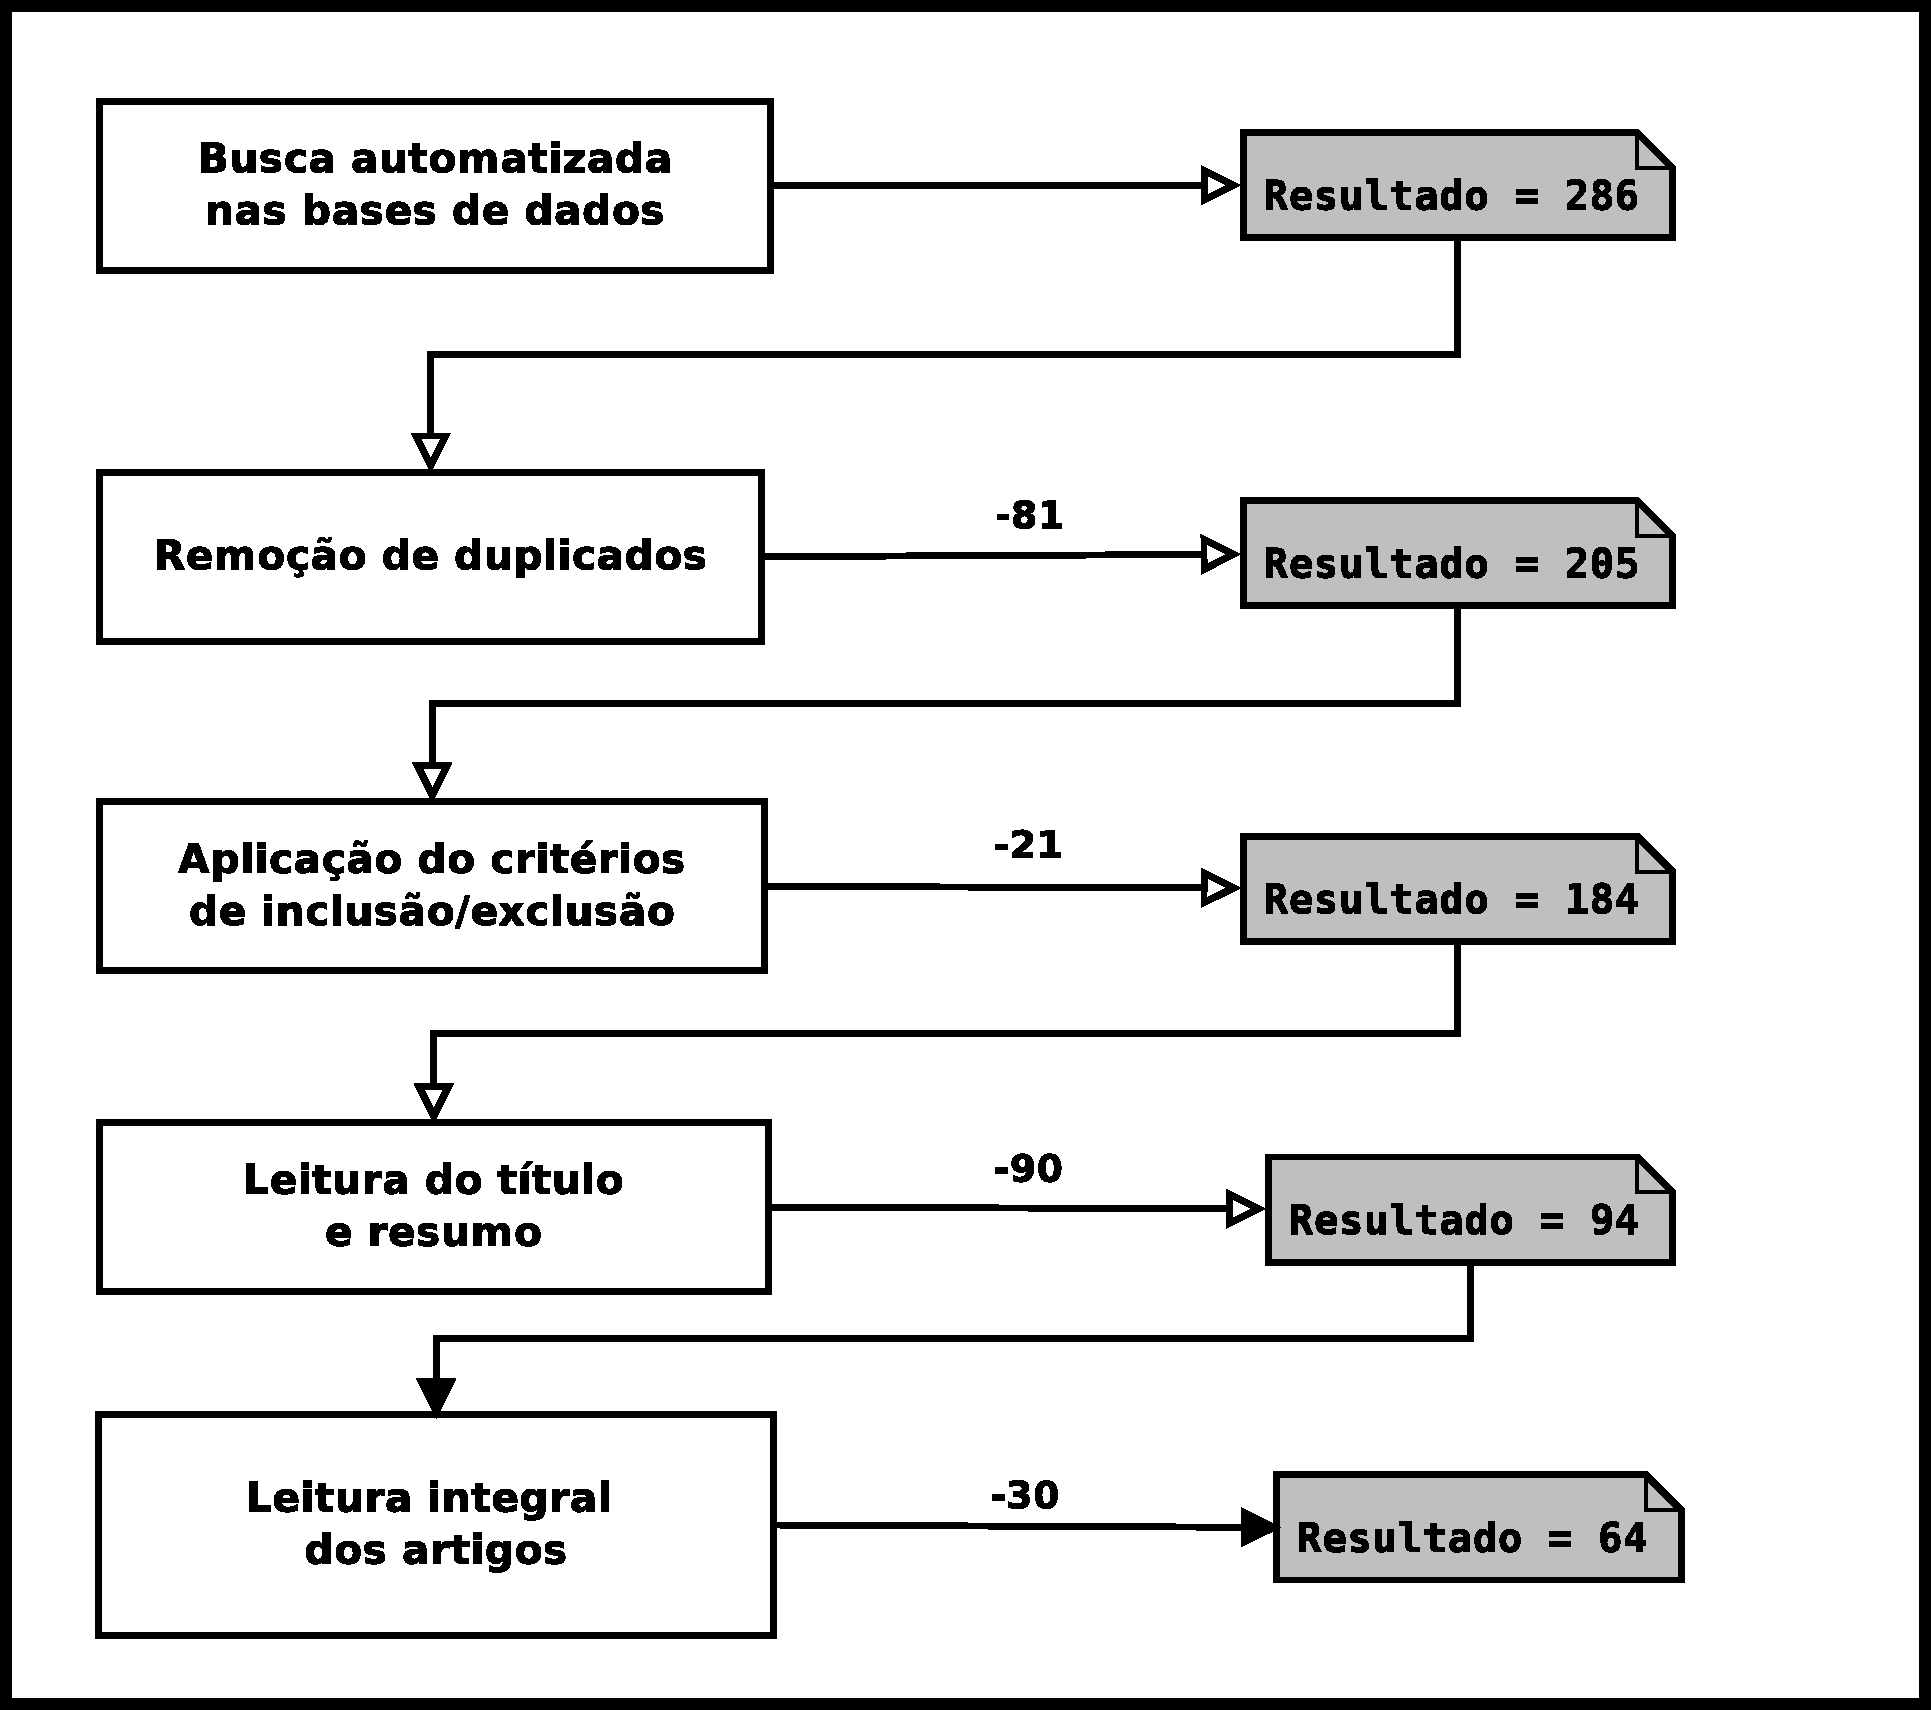
\includegraphics[width=0.75\linewidth]
	{./chapter-mapeamento-sistematico/img/diagrama-processo-selecao.pdf}
	\caption{Número de artigos incluídos durante o processo de seleção dos
		estudos. Baseado
		em~\cite{Petersen2015}}\label{fig:diagrama-processo-selecao}
\end{figure}

\begin{table}[htb]
	\centering
	\caption{Número de Estudos Recuperados por Base de Dados}\label{tab:estudos-por-base-dados}
	\begin{tabular}{cc}
		\hline
		\textbf{Base de Dados} & \textbf{Total} \\ \hline
		ACM Digital Library    & 109            \\
		IEEE Explore           & 100            \\
		Inspec/Compendex       & 22             \\
		Scopus                 & 55             \\ \hline
	\end{tabular}

\end{table}

\subsection{Esquemas de Classificação}
\label{subsec:map-esquemas-classificacao}

Com o objetivo de mapear os estudos sobre extensões das FGRM's foram propostos
quatro esquemas de classificação. O primeiro esquema organiza os artigos pelo
tipo de problema da atividade de manutenção de software a extensão se propõe
solucionar. A segunda categorização distribuí os estudos pelo papel no processo
de manutenção de software a extensão visa dar suporte. A terceira é uma
classificação baseada na taxonomia para modelos de Recuperação da Informação
(Information Retrieve~-~IR) proposta por Cerulo e
Canfora~\cite{cerulo2004taxonomy}. Em particular, utilizamos este esquema tendo
em vista que grande parte das extensões propostas na literatura utilizam algum
tipo de suporte de modelos de IR\@. O último esquema apresenta quais das
ferramentas existentes na indústria estão sendo estendidas na literatura. Esta
taxonomia nos fornece uma visão se as extensões propostas são com um foco
propositivo, ou seja, sem que exista uma implementação concreta da extensão, ou
se há algum tipo de ferramenta no qual existe um maior número de extensões
propostas. Em seguida discutiremos cada esquema de classificação em detalhe.

\subsubsection{Classificação por Tipo de Problema}
\label{subsubsec:map-esquema-suporte-problema}

Existem diversos problemas relacionados ao processo de Manutenção de Software.
Já na década de 1980 pesquisas questionavam os profissionais envolvidos com
manutenção de software quais os principais problemas da
área\cite{Lientz:1981:PAS:358790.358796}. Naturalmente a percepção dos desafios
envolvidos com a manutenção de software se altera com tempo, desta forma, é
sempre válido revisar a literatura com o objetivo de entender quais os tipos de
problemas estão sendo estudados.

Neste sentido foi proposto um esquema de classificação que relaciona os estudos
pelo tipo de problema que a extensão pretende resolver. A construção da
taxonomia se deu com base no processo definido por Petersen e
outros~\cite{Petersen2008}, o qual é composto de duas etapas:

\begin{enumerate}[I]
	\item analisar as palavras-chaves e conceitos que identificam as
		contribuições do estudo por meio da analise do título e resumo
	\item após o término da etapa I, todas as palavras chaves são combinadas a
		fim de construir um conjunto de categorias para no qual os artigos devem
		ser classificados.
\end{enumerate} 

Os autores recomendam que nos casos em que o resumo e o título do estudo não
sejam capazes de caracterizá-lo, as seções de introdução e conclusão também
devem ser analisadas. Para as bases de dados onde era informado mais de um
conjunto de palavras-chaves para um mesmo artigo, utilizamos aquelas que foram
informadas pelos autores. Mediante a aplicação do processo foi construído o
esquema de classificação apresentado na
Figura~\ref{fig:diagrama-esquema-dimensao-melhorias}.

\begin{figure}[tb]
\centering
 \makebox[\textwidth]{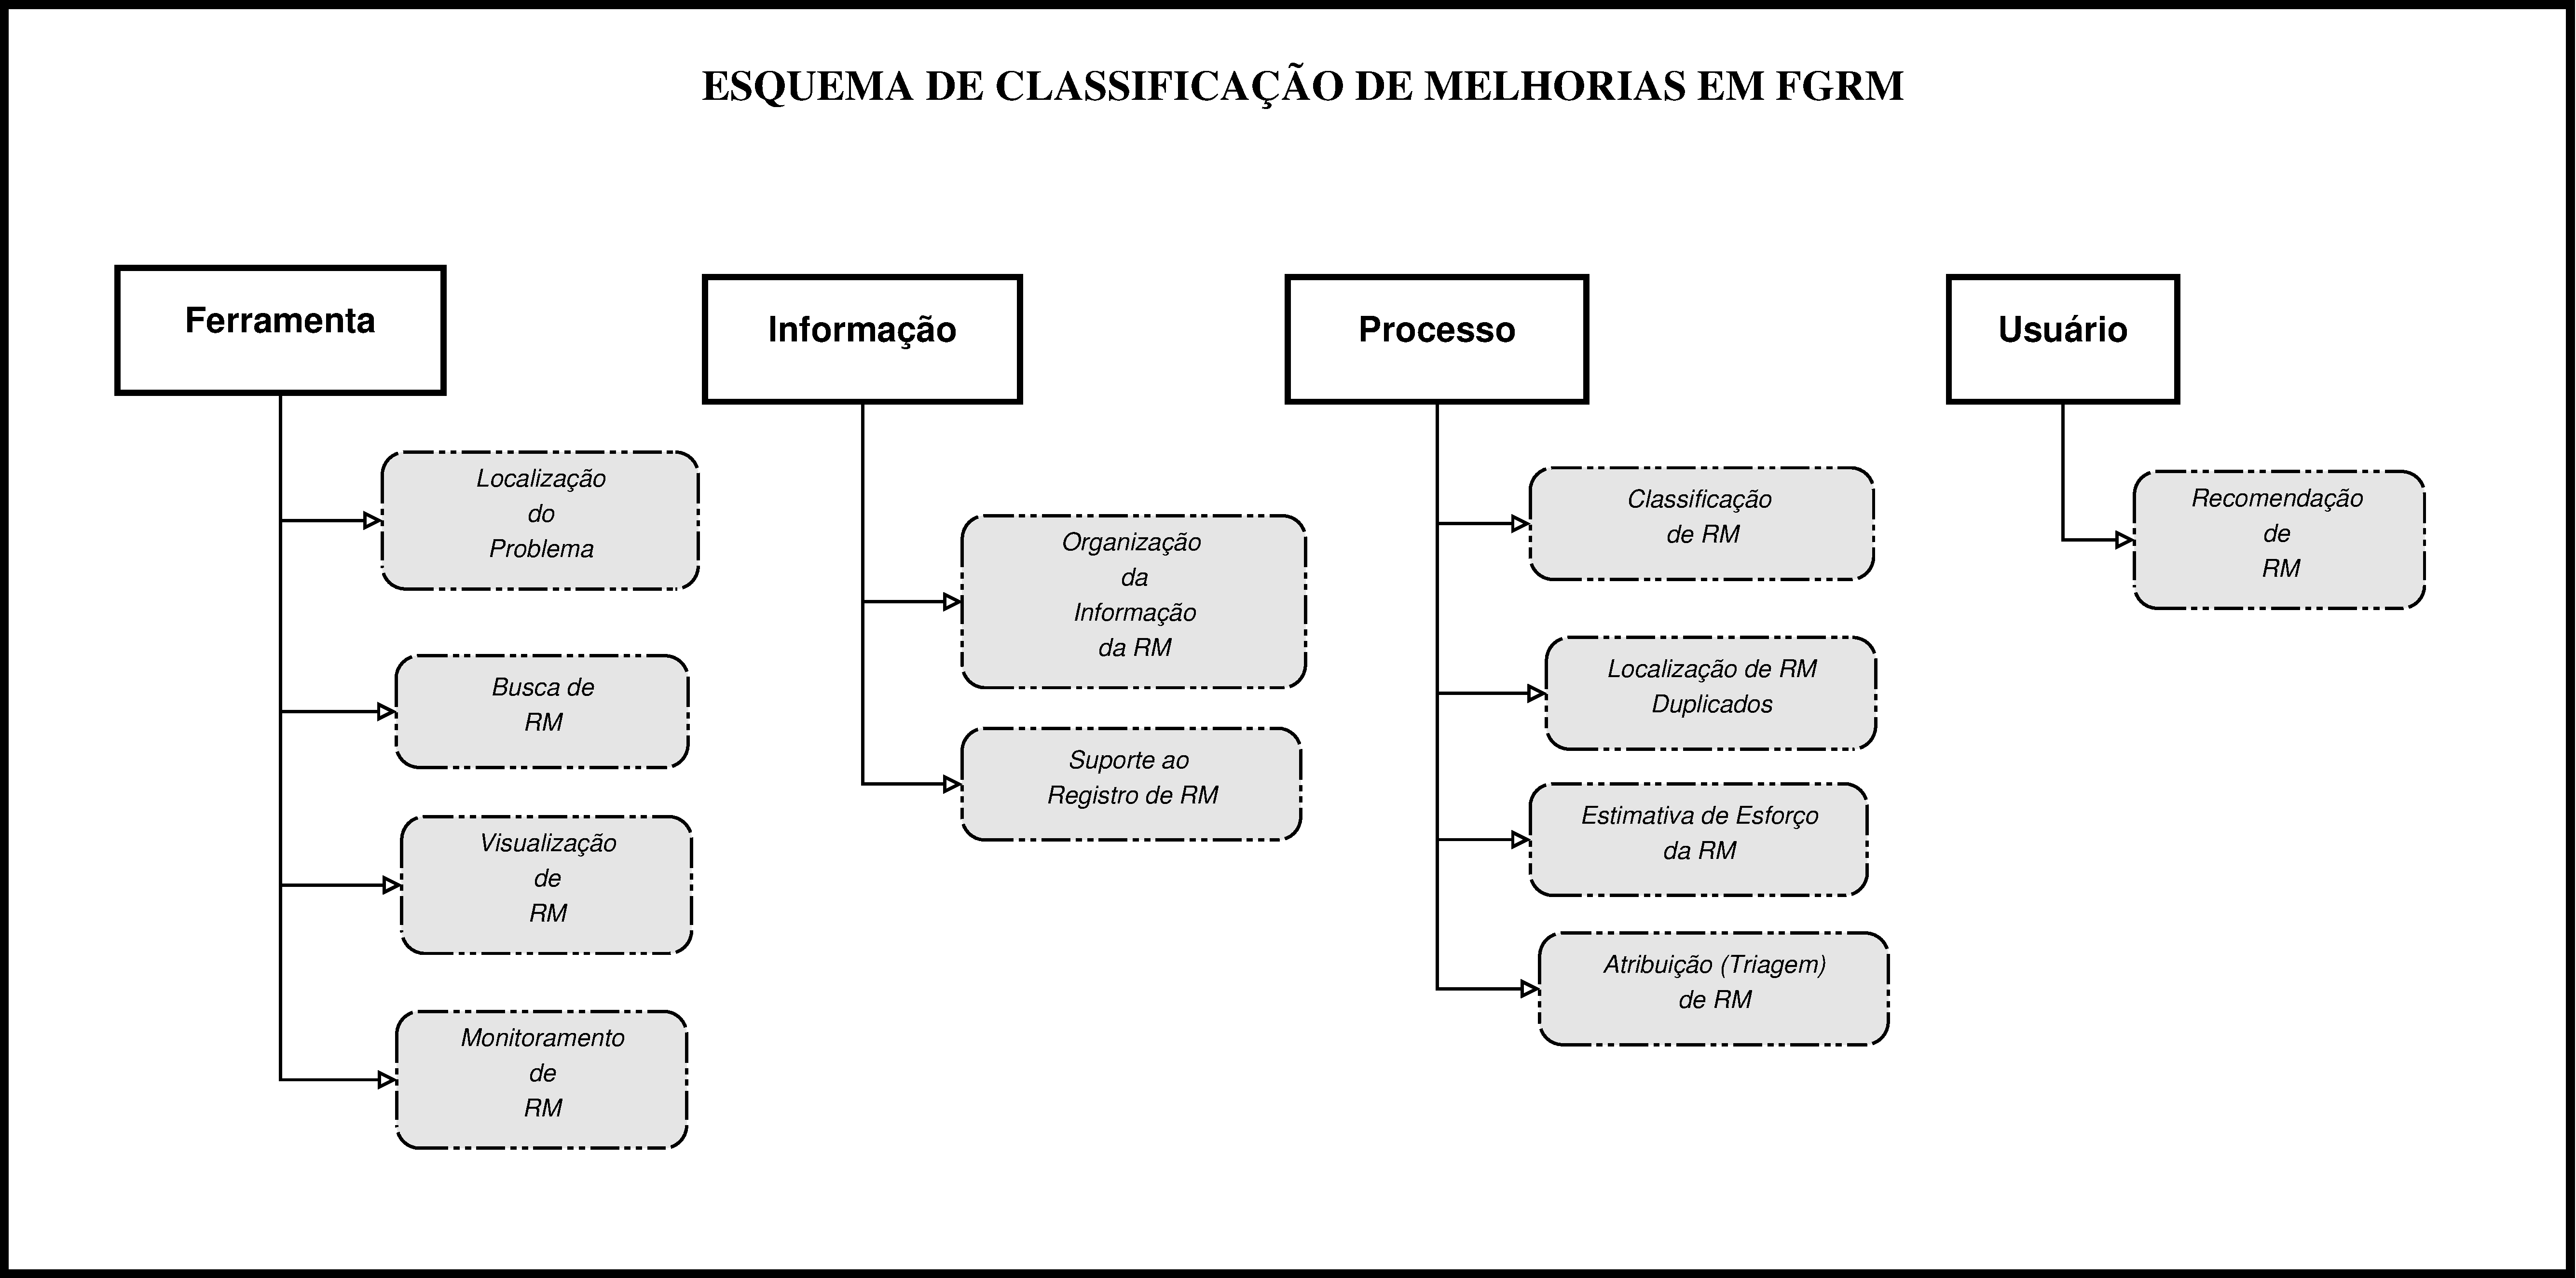
\includegraphics[width=.9\paperwidth]{./chapter-mapeamento-sistematico/img/diagrama-esquema-dimensoes-melhorias.pdf}}
\caption{Esquema de classificação das melhorias propostas na litetura. Os
	retângulos representam as dimensões de melhorias e os polígonos de cantos
	arredondados represetam as melhorias.}
\label{fig:diagrama-esquema-dimensao-melhorias}
\end{figure}
\todo[inline]{Incluir no anexo uma tabela demonstrando como as palavras-chaves foram combinadas}



\subsubsection{Classificação por Suporte ao Papel da Manutenção de Software}
\label{subsubsec:map-esquema-suporte-papel-man}

Da mesma forma que uma extensão proposta para as FGRM's visa resolver
determinado problema, supomos ainda que a extensão pode dar suporte a
determinado papel desempenhado no processo de Manutenção de Software. Para este
fim utilizamos uma classificação modificada da proposta por~\cite{Polo1999}. No
trabalho de Polo e outros o objetivo era definição de uma estrutura adequada da
equipe de manutenção de software mediante a clara identificação das tarefas que
cada membro deve executar. Os papéis propostos pelo no estudo é produto da
aplicação da metodologia MANTEMA~\cite{756695} para manutenção em projetos de
software bancários espanhóis, em especial aqueles em que a área de manutenção
foi terceirizada (outsourcing). Os autores reforçam que apesar da taxonomia de
papéis ter sido criada em um contexto específico, ela pode ser adequada para
aplicação em outras situações.

No escopo deste trabalho a taxonomia utiliza a proposta de Polo e outros com
algumas adequações. Em especial, foram removidos os papéis que segundo o nosso
entendimento estão mais vinculados a um contexto de manutenção terceirizada
(outsourcing). Além disso, dividimos o papel ``time de manutenção' (maintenance
team) em \textit{Desenvolvedor e Analista de Qualidade} por entendemos que são
papéis comuns a muito dos processos de manutenção existentes. Os papéis que
compõe a taxonomia proposta estão descritos a seguir:

\begin{description}
	\item[Usuário Afetado]: Indivíduo que utiliza o sistema do qual será
		produzida uma Requisição de Mudança.
	\item[Reportador]: Responsável por registrar a Requisição de Mudança na
		FGRM\@.
	\item[Gerente de Requisição de Mudança (Maintenance-request manager)]:
		Responsável por decidir se uma Requisição de Mudança será aceita ou
		rejeitada e qual tipo de manutenção deverá ser aplicada. Posteriormente
		cabe a ele/ela encaminhar a RM para o Agendador.
	\item[Agendador (Scheduler)]: Deve planejar a fila de Requisições de Mudança
		aceitas. Também estão no rol de responsabilidades deste papel a
		atribuição das RM's para o desenvolver mais apto.
	\item[Desenvolvedor]: Responsável realizar as ações que irão solucionar a
		Requisição de Mudança.
	\item[Analista de Qualidade]: Avaliam uma Requisição de Mudança que foi
		solucionada por um Desenvolvedor afim de verificar se a RM foi
		corretamente resolvida.
	\item[Líder da Manutenção (Head of Maintenance)]: Tem por responsabilidade
		definir os padrões e procedimentos que compõe o processo de manutenção
		que será utilizado.
\end{description}

Apesar da taxonomia de papéis utilizada derivar de um contexto de manutenção de
software específico (setor bancário e empresas com a área de manutenção
terceirizada), ela é capaz de acoplar com outros tipos de processo de manutenção
de software, como aquele proposto por Ihara e outros
\cite{Ihara:2009:AMI:1595808.1595833}. Naquele estudo foi criada uma
representação de um processo de modificação de bugs tomando como base as
diversas situações que um bug possui em uma FGRM no contexto de projetos de
código aberto. O processo resultante é facilmente acoplável com a taxonomia
utilizada em nosso estudo.

Cabe ressaltar que está fora do escopo deste estudo elaborar uma taxonomia de
papeis envolvidos na Manutenção de Software em função de supormos que isto
corresponde a um esforço bem extenso. Nossa ação é identificar quais artigos
trabalham com a noção de quais papeis a extensão pretender dar suporte,  ou
seja,  relatar se existem papeis e quais são eles,  sem com isso, envolver em
uma consolidação definitiva.

\subsubsection{Classificação por Técnicas de Recuperação da Informação}
\label{subsubsec:map-esaquema-tecnicas-ir}

Um ponto em comum entre as diversas extensões para FGRM propostas na literatura
é o fato delas utilizarem algum suporte de modelos de Recuperação de Informação
(Information Retrieve~-~IR). Um modelo de IR visa solucionar um uma necessidade
informacional de um usuário, representada como um conjunto de termos, no qual
uma lista dos documentos mais relevantes devem ser recuperadas de uma
coleção~\cite{baeza1999modern}. 

Com o objetivo de obter uma visão geral das técnicas que estão sendo utilizadas
para implementar as extensões para as FGRM, realizamos a classificação dos
estudos através da taxonomia proposta por Canfora e
Cerulo\cite{cerulo2004taxonomy}. O esquema de classificação consiste em duas
visões sobrepostas: uma taxonomia vertical que classifica os modelos de IR com
relação ao seu conjunto de características básicas; e uma taxonomia horizontal
que classifica os objetos de IR com respeito as suas tarefas, forma e
contexto\cite{cerulo2004taxonomy}. Nesta dissertação utilizamos a classificação
vertical tendo em vista que estamos interessados na técnica utilizada na
implementação da extensão.

\todo[inline]{Verificar a necessidade de definir melhor alguns termos de IR\@.
	Ex\@. documento, consulta do usuário, problema da representação de
	similaridade}

\todo[inline]{Verificar o total de artigos que utilizam algum técnica de IR\@.
	Apesar de grande parte utilizar não serão todos os artigos}

A taxonomia vertical é construída explorando duas características básicas de um
Modelo de Recuperação da Informação: \textit{representação (representation)},
que é a forma adotada para representar ao mesmo tempo o documento e consulta do
usuário; \textit{raciocínio (reasoning)}, ao qual se refere ao framework adotado
para resolver o problema da representação de similaridade, ou seja, trata-se do
conjunto de métodos, modelos e tecnologias utilizadas para realizar o casamento
entre um documento e a consulta do usuário. O esquema de classificação proposto
pelos autores é apresentado na Figura~\ref{fig:information-retrieval-model}.

\begin{figure}[htpb]
	\centering
	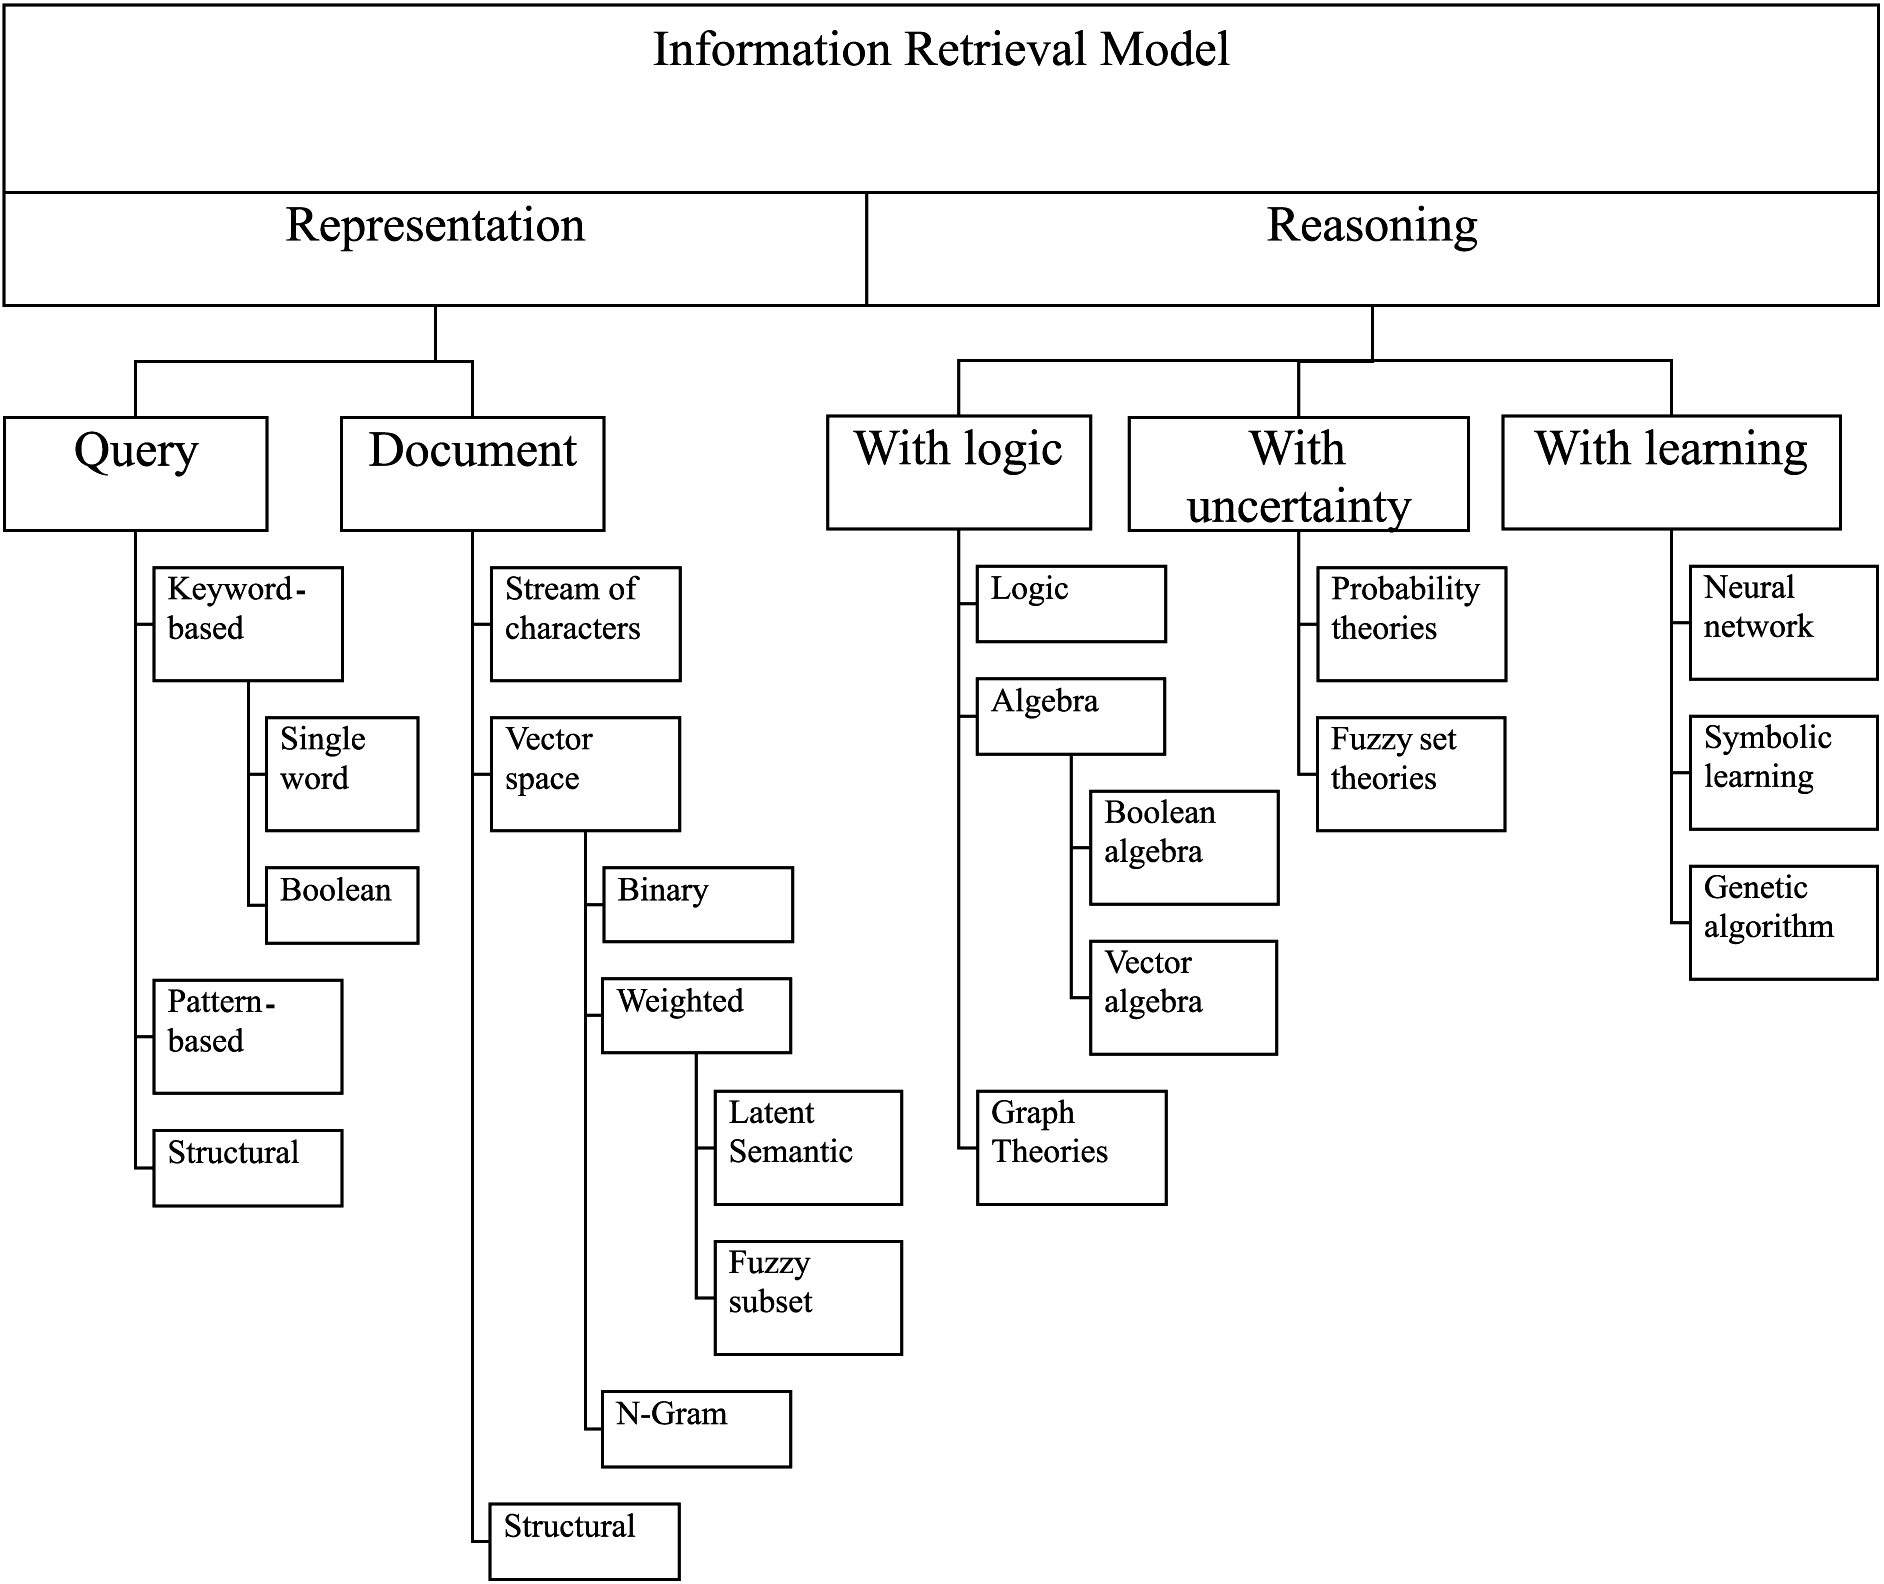
\includegraphics[width=0.8\linewidth]{./chapter-mapeamento-sistematico/img/information-retrieval-model.png}
	\caption{Taxonomia vertical para Modelos de Recuperação da Informação.
		Adaptado
		de~\cite{cerulo2004taxonomy}}\label{fig:information-retrieval-model}
\end{figure}

\subsubsection{Classificação por Ferramenta Estendida}
\label{subsubsec:map-esquema-ferramenta}

Do ponto de vista dos profissionais envolvidos em Manutenção de Software é
importante entender quais as FGRM estão sendo estendidas. Por outro lado, para
os pesquisadores é importante descobrir aquelas ferramentas mais ``amigáveis
para o desenvolvimento de novas extensões bem como a melhoria das existentes.
Neste sentido, realizamos a classificação dos estudos pelas ferramentas que
foram utilizados para o desenvolvimento das extensões. Uma ferramenta é
entendida como utilizada por determinado estudo se ela foi utilizada no processo
de validação ou se seus dados foram utilizados na avaliação da extensão. 

Para produzirmos a taxonomia realizarmos a leitura do resumo e da introdução do
artigo. Nos casos em que não foi possível determinar a ferramenta utilizada a
partir da leitura das seções citadas, procedemos com a leitura com a parte
avaliação do estudo. A Tabela exibe as ferramentas utilizadas para cada estudo
analisado.

\section{Resultados}
\label{sec:resultados}

Nesta seção apresentamos os resultados do Mapeamento Sistemático. Cada uma das
taxonomias propostas é analisada mediante a apresentação dos estudos que possam
exemplificar a classificação adotada.  Iniciamos com uma análise da frequência
de publicação relativo à melhoria das funcionalidades das ferramentas.
Posteriormente apresentamos os resultados pela classificação por problemas na
Manutenção de Software, o qual dividimos os estudos por área e tópico de
pesquisa. Seguimos com a análise dos estudo pelo papel ao qual a extensão visa
dar suporte. Posteriormente analisamos os modelos de IR utilizados para
implementar algumas das extensões propostas na literatura. Finalizamos esta
análise com as ferramentas existentes no mercado que estão efetivamente sendo
entendidas.

\subsection{Frequência das Publicações}
\label{sub:frequencia_publicacao}

A Figura~\ref{fig:publicacao_por_ano} exibe o número de estudos primários
identificados entre os anos 2010-2016, período de referência utilizado no
mapeamento. Dentre os estudos escolhidos no período em questão verificamos que
em 2010 foram publicados cinco estudos sobre o assunto
\cite{sun2010discriminative,gegick2010identifying,song2010jdf,nagwani2010predictive,zimmermann2010makes}.
Posteriormente verificamos um acréscimo no número de estudos no qual um
significante aumento pode ser observado entre os anos de 2012-2014. O crescente
número de estudos publicados sobre melhorias nas FGRM pode indicar que esta área
vem sendo considerada altamente relevante pela comunidade acadêmica em
Engenharia de Software.

\begin{figure}[htpb]
	\centering
	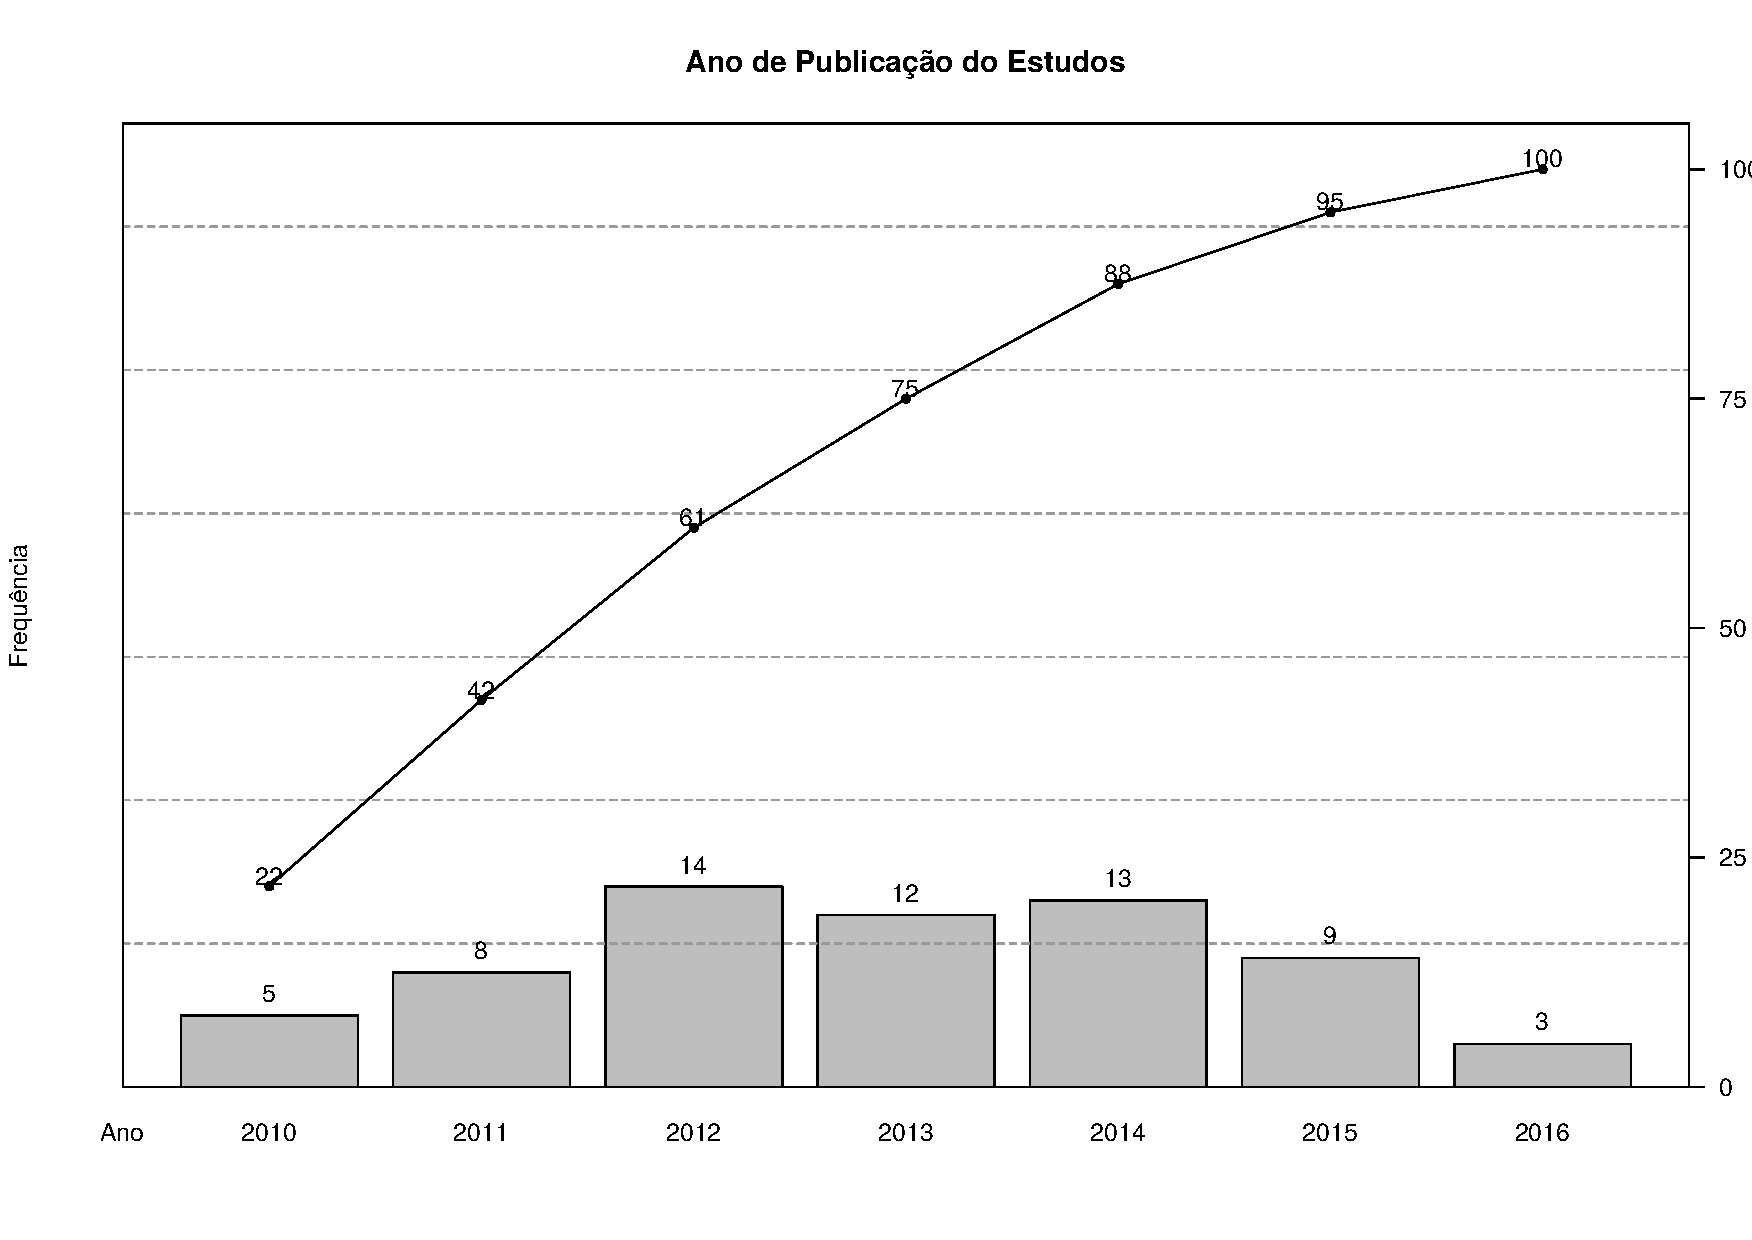
\includegraphics[width=0.9\linewidth]{chapter-mapeamento-sistematico/img/ano-publicao-estudos.pdf}
	\caption{Número de estudos primários por ano de publicação.}
	\label{fig:publicacao_por_ano}
\end{figure}

\subsection{Extensões para Problemas na Manutenção de Software}
\label{sub:extensões_para_problemas_na_manutenção_de_software}

Nesta etapa do trabalho estamos interessados no estado da arte do estudo dos
problemas encontrados na Manutenção de Software. Em especial, o nosso foco é
entender que tipo de melhorias nas funcionalidades das FGRM estão sendo proposta
na literatura. Com base no mapeamento sistemático realizado e nas dimensões de
melhoria discutidas por Zimmermann e outros~\cite{5070993} construímos o esquema
de classificação dos apresentado na
Figura~\ref{fig:diagrama-esquema-dimensao-melhorias}

Adicionalmente a tabela~\ref{tab:taxonomia-problemas-manutencao} exibe a
distribuição dos estudos pela dimensaõ de melhoria e o seu respetivo tópico. De
uma certa maneira o número de estudos  pode indicar a maturidade da pesquisa
naquele tipo de assunto. Contudo, não representa diretamente a importânica do
tópico no estudo sobre melhorias em FGRM's.

% Inclusão da tabela
\begin{table}[htbp]
\centering
\caption{My caption}
\label{my-label}
\resizebox{\textwidth}{!}{%
\begin{tabular}{|c|l|l|c|}
\hline
\textbf{Dimensão da Melhoria} & \multicolumn{1}{c|}{\textbf{Tópico}}             & \multicolumn{1}{c|}{\textbf{Estudos}}          & \textbf{Total}       \\ \hline
\multirow{13}{*}{Ferramenta}  & Busca de RM                                      & \cite{Liu2014}                                 & 1                    \\ \cline{2-4} 
                              & \multirow{7}{*}{Localização do Problema}         & \cite{Bangcharoensap:2012:LSC:2419061.2419428} & \multirow{7}{*}{7}   \\
                              &                                                  & \cite{Corley2011}                              &                      \\
                              &                                                  & \cite{Nguyen:2012:MAR:2393596.2393671}         &                      \\
                              &                                                  & \cite{Romo:2015:TAT:2745802.2745833}           &                      \\
                              &                                                  & \cite{thung2013automatic}                      &                      \\
                              &                                                  & \cite{Thung:2014:BIT:2635868.2661678}          &                      \\
                              &                                                  & \cite{Wong:2014:BBF:2705615.2706096}           &                      \\ \cline{2-4} 
                              & Monitoramento de RM                              & \cite{Aggarwal:2014:MIT:2593801.2593810}       & 1                    \\ \cline{2-4} 
                              & \multirow{4}{*}{Visualização de RM}              & \cite{dal2013closer}                           & \multirow{4}{*}{4}   \\
                              &                                                  & \cite{Hora2012}                                &                      \\
                              &                                                  & \cite{Sasso2014}                               &                      \\
                              &                                                  & \cite{takama2013application}                   &                      \\ \hline
\multirow{9}{*}{Informação}   & \multirow{2}{*}{Organização da Informação da RM} & \cite{mani2012ausum}                           & \multirow{2}{*}{2}   \\
                              &                                                  & \cite{Otoom2016}                               &                      \\ \cline{2-4} 
                              & \multirow{7}{*}{Suporte ao Registro da RM}       & \cite{Bettenburg2008a}                         & \multirow{7}{*}{7}   \\
                              &                                                  & \cite{Correa2013b}                             &                      \\
                              &                                                  & \cite{moran2015auto}                           &                      \\
                              &                                                  & \cite{Moran:2015:EAA:2786805.2807557}          &                      \\
                              &                                                  & \cite{Tu:2014:MQI:2677832.2677844}             &                      \\
                              &                                                  & \cite{White:2015:GRR:2820282.2820291}          &                      \\
                              &                                                  & \cite{Wu2011a}                                 &                      \\ \hline
\multirow{40}{*}{Processo}    & \multirow{12}{*}{Atribuição (Triagem) de RM}     & \cite{Banitaan2013}                            & \multirow{12}{*}{12} \\
                              &                                                  & \cite{hosseini2012market}                      &                      \\
                              &                                                  & \cite{Hu:2014:EBT:2707683.2708297}             &                      \\
                              &                                                  & \cite{Naguib2013}                              &                      \\
                              &                                                  & \cite{Nagwani2012}                             &                      \\
                              &                                                  & \cite{shokripour2012automatic}                 &                      \\
                              &                                                  & \cite{tian2015automated}                       &                      \\
                              &                                                  & \cite{ValdiviaGarcia:2014:CPB:2597073.2597099} &                      \\
                              &                                                  & \cite{Wu2011}                                  &                      \\
                              &                                                  & \cite{Xuan:2012:DPB:2337223.2337227}           &                      \\
                              &                                                  & \cite{Zanetti2013}                             &                      \\
                              &                                                  & \cite{Zhang2014}                               &                      \\ \cline{2-4} 
                              & \multirow{10}{*}{Classificação de RM}            & \cite{behl2014bug}                             & \multirow{10}{*}{10} \\
                              &                                                  & \cite{chawla2015automated}                     &                      \\
                              &                                                  & \cite{Gegick2010}                              &                      \\
                              &                                                  & \cite{Izquierdo2015}                           &                      \\
                              &                                                  & \cite{kochhar2014automatic}                    &                      \\
                              &                                                  & \cite{Nagwani2013}                             &                      \\
                              &                                                  & \cite{netto2010automated}                      &                      \\
                              &                                                  & \cite{somasundaram2012automatic}               &                      \\
                              &                                                  & \cite{Tian:2013:DPP:2550526.2550574}           &                      \\
                              &                                                  & \cite{zhang2011bug}                            &                      \\ \cline{2-4} 
                              & \multirow{5}{*}{Estima de Esforço da RM}         & \cite{Bhattacharya:2011:BTP:1985441.1985472}   & \multirow{5}{*}{5}   \\
                              &                                                  & \cite{Nagwani2010}                             &                      \\
                              &                                                  & \cite{Thung2012}                               &                      \\
                              &                                                  & \cite{Vijayakumar2014}                         &                      \\
                              &                                                  & \cite{xia2015automatic}                        &                      \\ \cline{2-4} 
                              & \multirow{13}{*}{Localização de RM Duplicados}   & \cite{alipour2013contextual}                   & \multirow{13}{*}{13} \\
                              &                                                  & \cite{banerjee2012automated}                   &                      \\
                              &                                                  & \cite{hindle2016contextual}                    &                      \\
                              &                                                  & \cite{Koopaei:2015:CAD:2886444.2886474}        &                      \\
                              &                                                  & \cite{Lerch:2013:FDY:2495256.2495763}          &                      \\
                              &                                                  & \cite{Liu:2012:TBR:2393596.2393628}            &                      \\
                              &                                                  & \cite{Prifti2011}                              &                      \\
                              &                                                  & \cite{Song2010a}                               &                      \\
                              &                                                  & \cite{sun2010discriminative}                   &                      \\
                              &                                                  & \cite{Sun2011}                                 &                      \\
                              &                                                  & \cite{Thung2014}                               &                      \\
                              &                                                  & \cite{Tian2012}                                &                      \\
                              &                                                  & \cite{Tomasev2013}                             &                      \\ \hline
\multirow{2}{*}{Usuário}      & \multirow{2}{*}{Recomendação de RM}              & \cite{malheiros2012source}                     & \multirow{2}{*}{2}   \\
                              &                                                  & \cite{Wang2011a}                               &                      \\ \hline
\end{tabular}%
}
\end{table}



\begin{figure}[tb]
\centering
 \makebox[\textwidth]{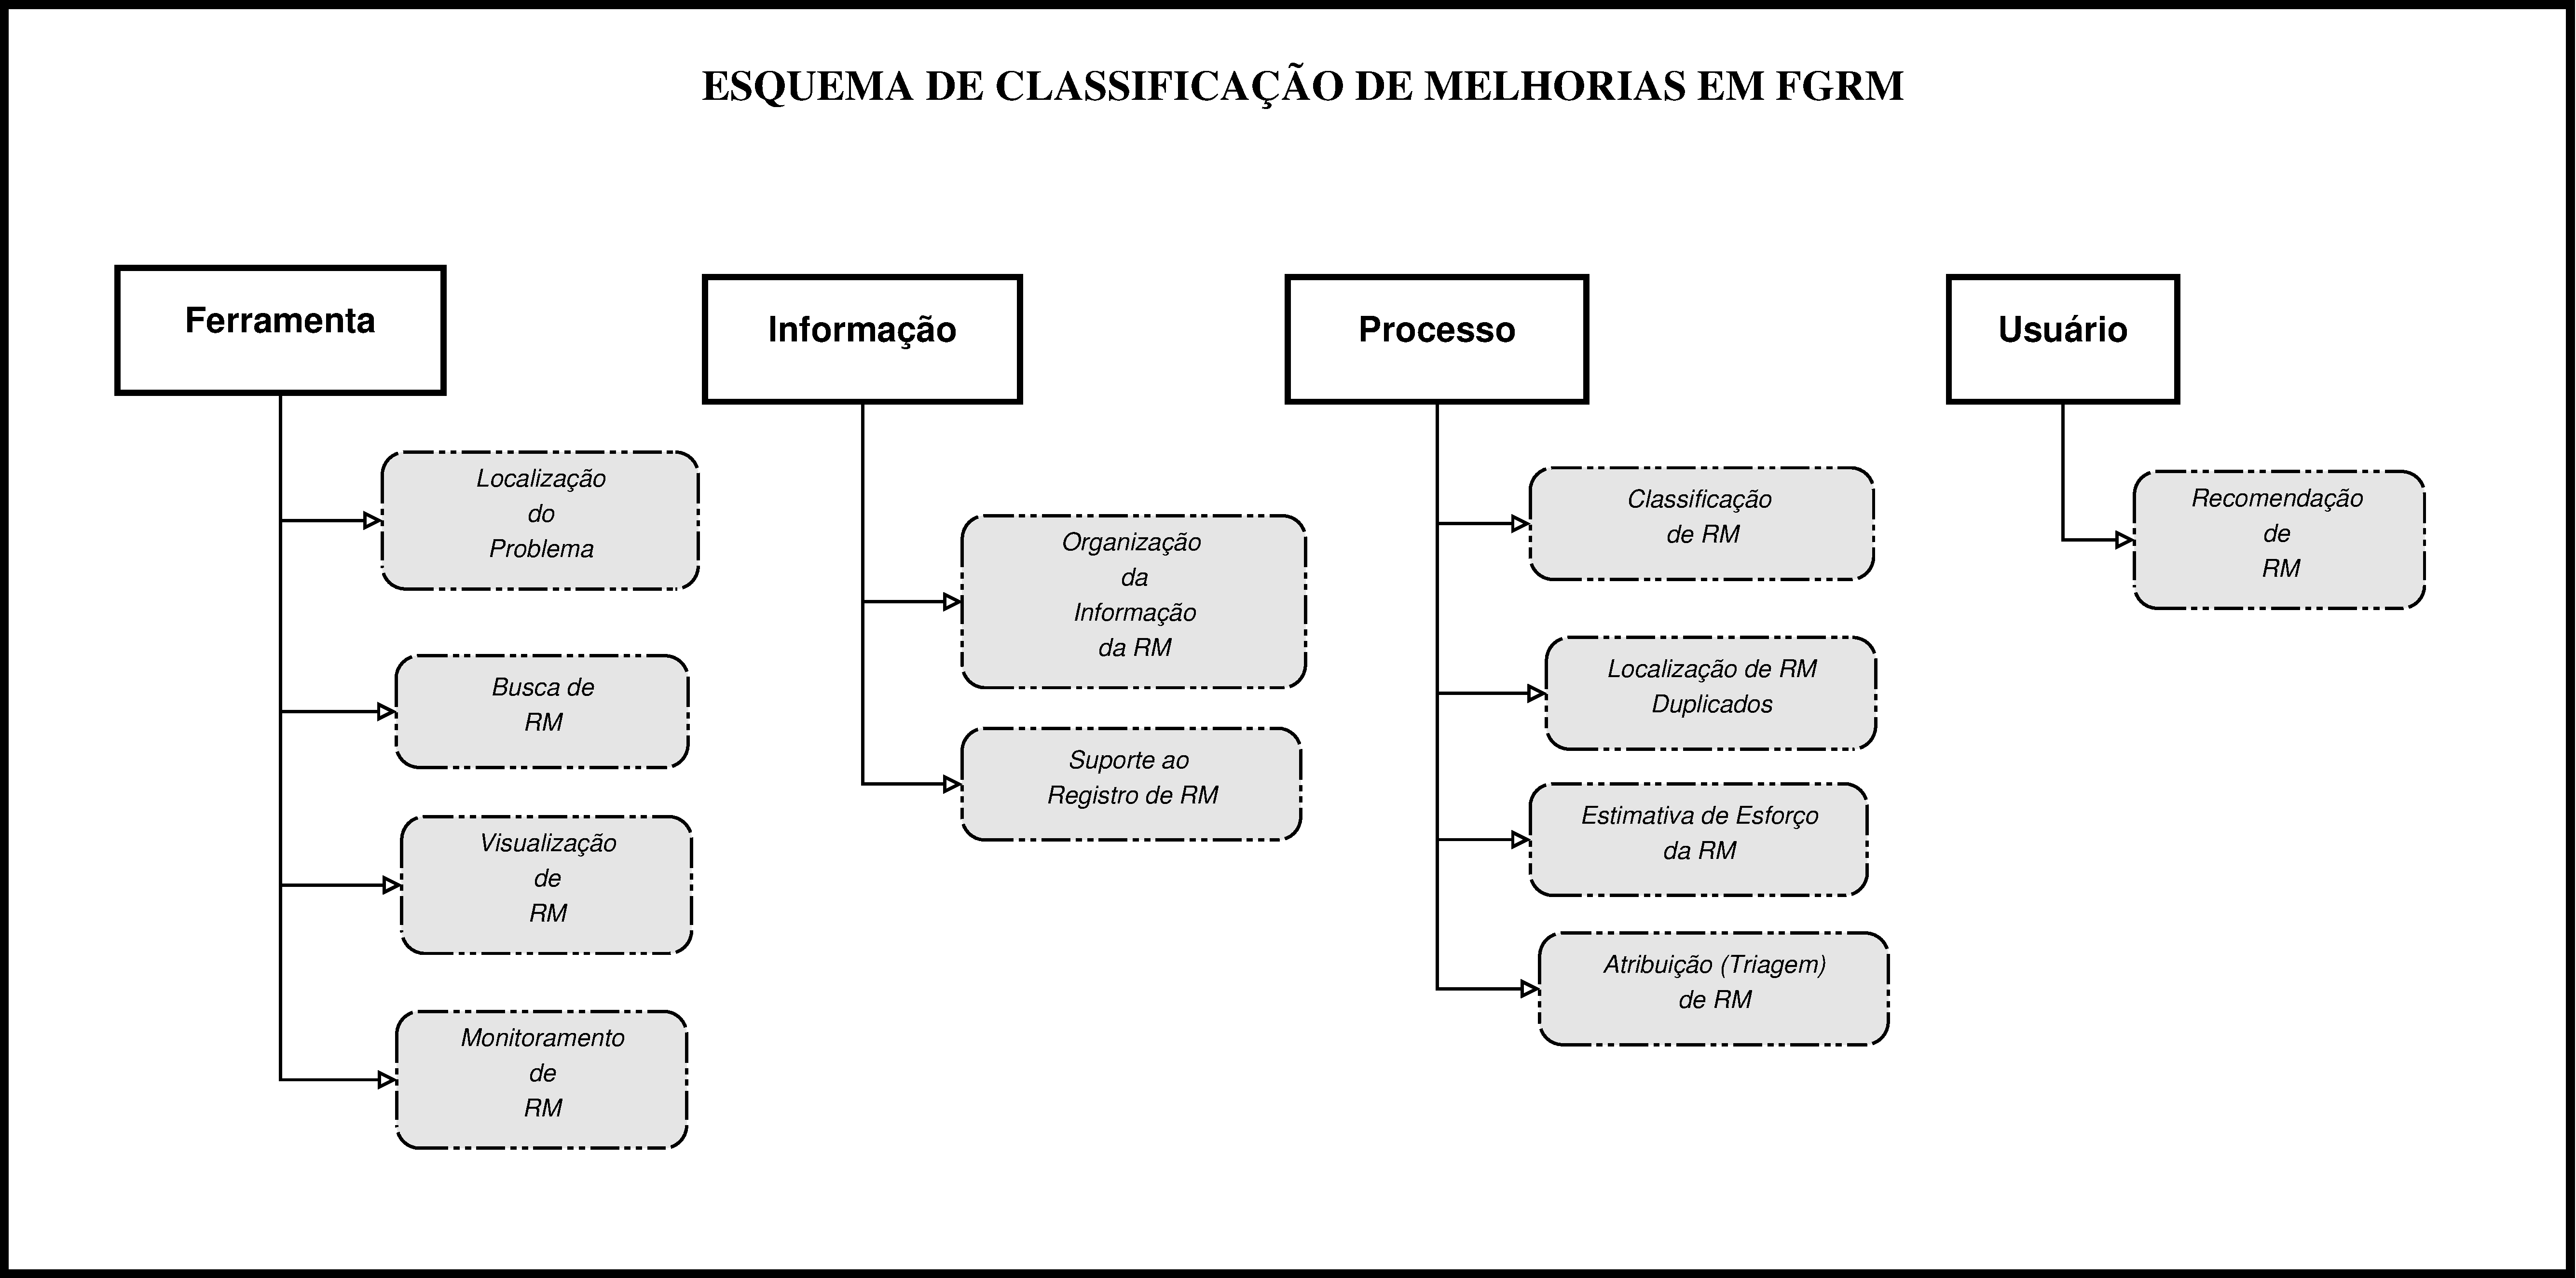
\includegraphics[width=.9\paperwidth]{./chapter-mapeamento-sistematico/img/diagrama-esquema-dimensoes-melhorias.pdf}}
\caption{Esquema de classificação das melhorias propostas na litetura. Os
	retângulos representam as dimensões de melhorias e os polígonos de cantos
	arredondados represetam as melhorias.}
\label{fig:diagrama-esquema-dimensao-melhorias}
\end{figure}

\begin{figure}[htpb]
	\centering
	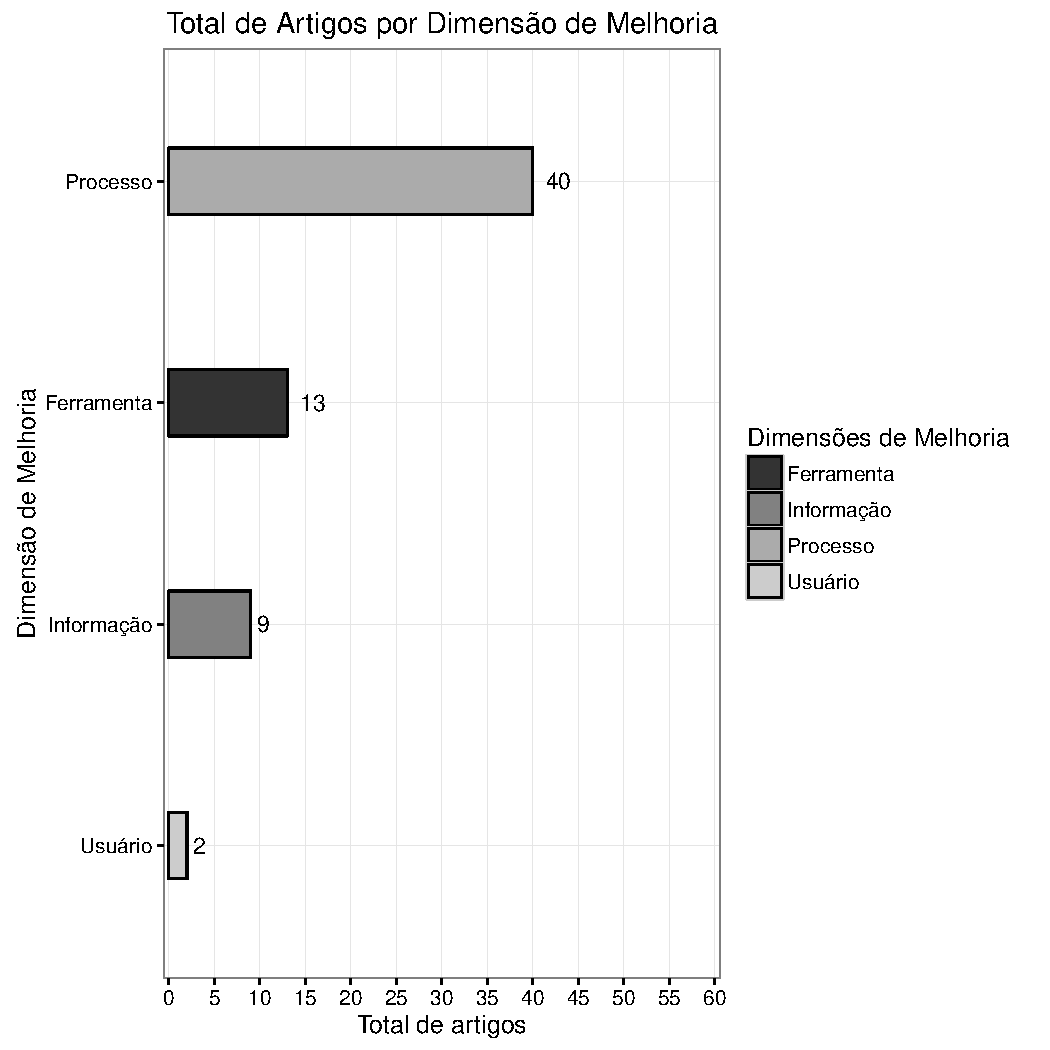
\includegraphics[width=0.9\linewidth]{./chapter-mapeamento-sistematico/img/grafico_dim_melhoria_por_artigo.pdf}
	\caption{Total de artigos por dimensão de melhoria}
	\label{fig:grafico_dim_melhoria_por_artigo}
\end{figure}


\subsubsection{Classificação de Requisições de Mudança}
\label{ssub:classificação_de_requisições_de_mudança}

\subsubsection{Duplicação}
\subsubsection{Categorização}
\subsubsection{Estimativa de Esforço}

\subsection{Extensões com Suporte à Papeis}
\label{sub:extensões_com_suporte_à_papeis}


\subsection{Técnicas de IR Utilizadas pelas Extensões}
\label{sub:técnicas_de_ir_utilizadaas_pelas_extensões}


\subsection{Ferramentais Estendidas}
\label{sub:ferrramentas_extendidas}


\section{Limitações e Ameaças à Validade}

\section{Trabalhos Relacionados}

\section{Resumo do Capítulo}